\documentclass[12pt,a4paper]{article}
\usepackage[parfill]{parskip}
\usepackage{fullpage}
\usepackage{enumitem}
\usepackage{hyperref}
\usepackage{graphicx}
\usepackage{subfig}
\usepackage{amsmath}
\begin{document}

\vfil

\begin{center}
	{\Large Mobile Robot Systems} \\
	\vspace{0.4in}
	{\huge \bf Assignment 2} \\
	\vspace{0.4in}
	{\large Anik Roy} \\
	\vspace{0.1in}
	{\large \today} \\
\end{center}
\vspace{0.4in}

% Main document

\section*{1.1 Potential Field Method}
\subsection*{Exercise 1}
\begin{enumerate}[label=(\alph*)]
	\item The plot of the potential field for moving towards the goal can be seen in figure \ref{fig:goal_mode}. This field is calculated by taking the vector from the position towards the goal, and squaring the magnitude of the vector while keeping the same direction. This ensures that the robot 'slows down' as it gets closer to the goal, and that it will always attempt to move towards the goal. The figure shows how all the vectors point towards the goal, and that vectors close to the goal have a smaller magnitude
	\begin{figure}[!h]
		\centering
		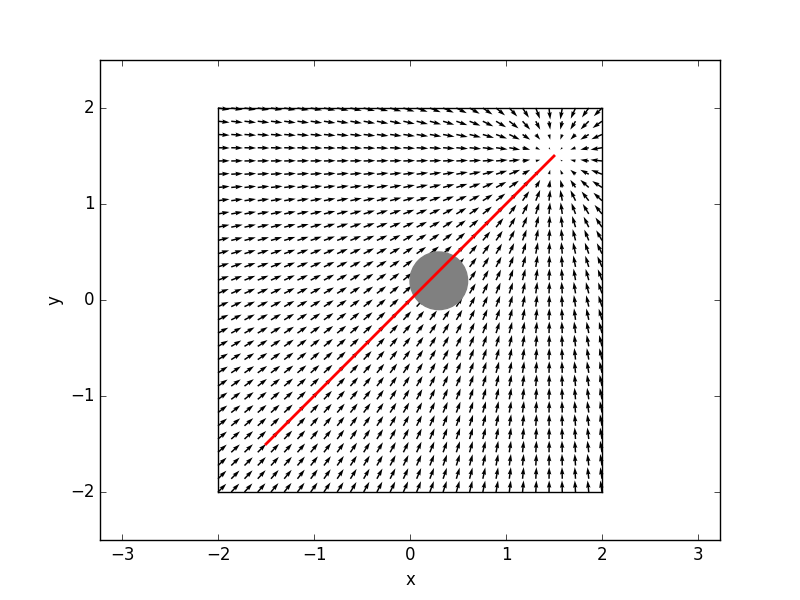
\includegraphics[width=\textwidth]{fig/1a.png}
		\caption{Potential field with the goal}
		\label{fig:goal_mode}
	\end{figure}
	\item In order to avoid obstacles, we also need to find a vector field which will let us move away from obstacles (a field that is repulsive). In order to do this, I first find the distance from the position to the surface of the  obstacle by finding the euclidean distance and subtracting the radius. Since positions closer to the obstacle should be more 'repulsive', the reciprocal of this distance is the magnitude of the final vector. The direction of the final vector is directly away from the centre of the obstacle towards the robot. I also scale this by a tunable parameter to ensure the robot makes progress. This process is repeated for each obstacle, and the vectors produced are summed so that all the obstacles are taken into account. The resulting vector is also capped to a maximum speed.
	\begin{figure}[!h]
		\centering
		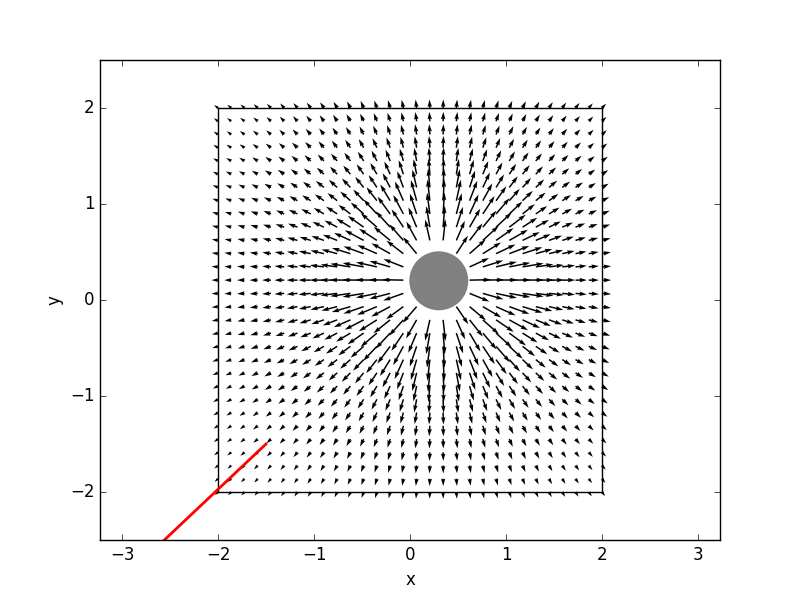
\includegraphics[width=\textwidth]{fig/1b.png}
		\caption{Potential field with the obstacles}
		\label{fig:obs_mode}
	\end{figure}
	\item Figure \ref{fig:all_mode} shows how combingin the two vector fields results in a new field which allows the robot to take a path to the goal while avoiding the obstacle. Since the vectors from the obstacle have a repulsive effect, and the vectors towards the goal have an attactive effect, they combine these effects to create vectors which go towards the goal but also away from the obstacle.
	\begin{figure}[!h]
		\centering
		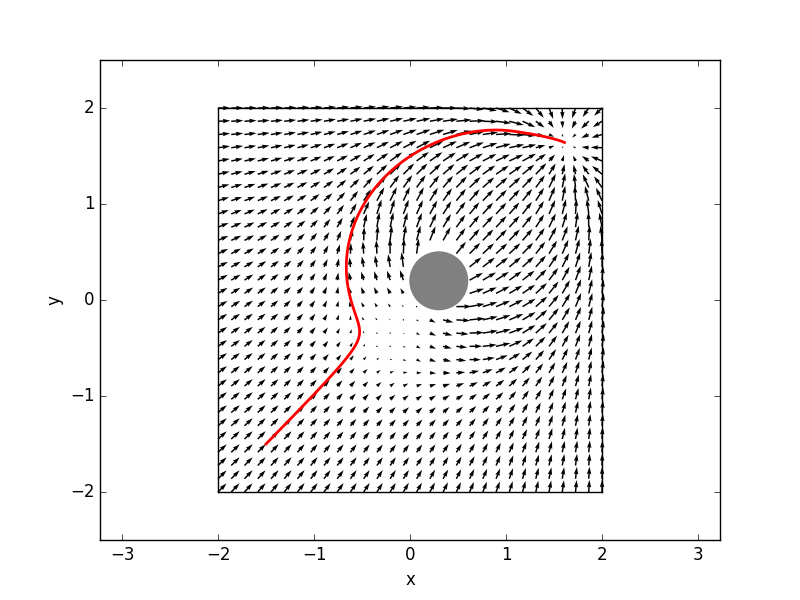
\includegraphics[width=\textwidth]{fig/1c.png}
		\caption{Potential field with both the goals and the obstacle}
		\label{fig:all_mode}
	\end{figure}
	\item In the previous part, the obstacle was at the position (0.2,0.3). Since the robot started at (-1.5,-1.5), and the vectors for the goal are direct, they will pass directly through the center of the obstacle. The vectors from the obstacle are in the opposite direction, as the direction of these vectors is the direction from the robot to the obstacle flipped. This means they will cancel each other out to produce a zero vector somewhere between the start position and the obstacle, stopping the robot. This can be seen in \ref{fig:failed_potential}, where the robot gets stuck halfway between the start and the obstacle. One possible solution is to change the direction of the vectors coming from the obstacle. Currently, they are directly in the direction of the robot, but they could be made to be skewed slightly so that the robot would always move in one direction. Once the robot moves in the direction, vectors towards the goal should allow the robot to keep moving. This still ensures the robot does not hit the obstacle, since the vectors are still repulsive, just in a slightly different direction.
	\begin{figure}[!h]
		\centering
		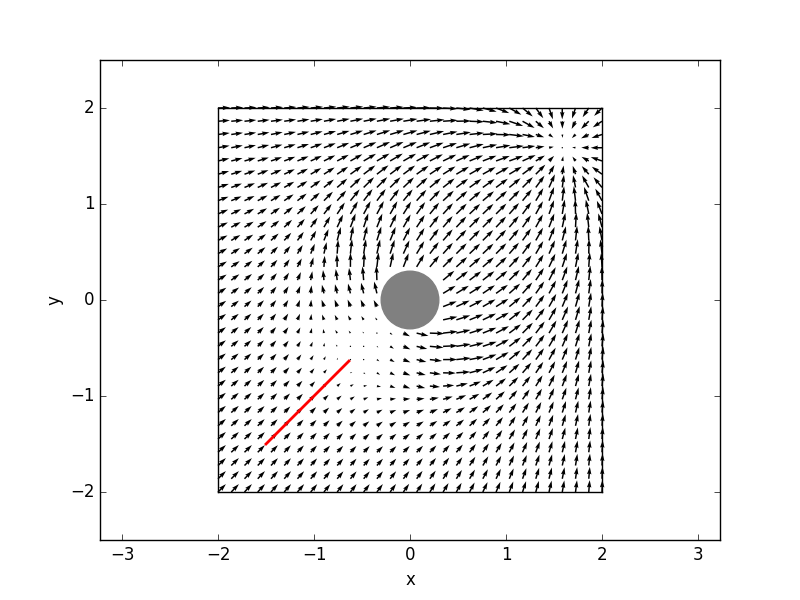
\includegraphics[width=\textwidth]{fig/1d.png}
		\caption{Potential field with the obstacle at (0,0)}
		\label{fig:failed_potential}
	\end{figure}
	\item Figure \ref{fig:fixed_potential} shows how the problem in part (d) can be fixed. The vectors coming from the obstacle are now rotated by 1 radian anti-clockwise (which can be tuned). This means that the robot will now take the path on the right of the obstacle, as it is pushed in that direction by these vectors. To calculate the vectors, I use the standard 2-D rotation matrix to ensure that the magnitude of the vector stays the same (it is rotated from its original direction around its base).
	\begin{figure}[!h]
		\centering
		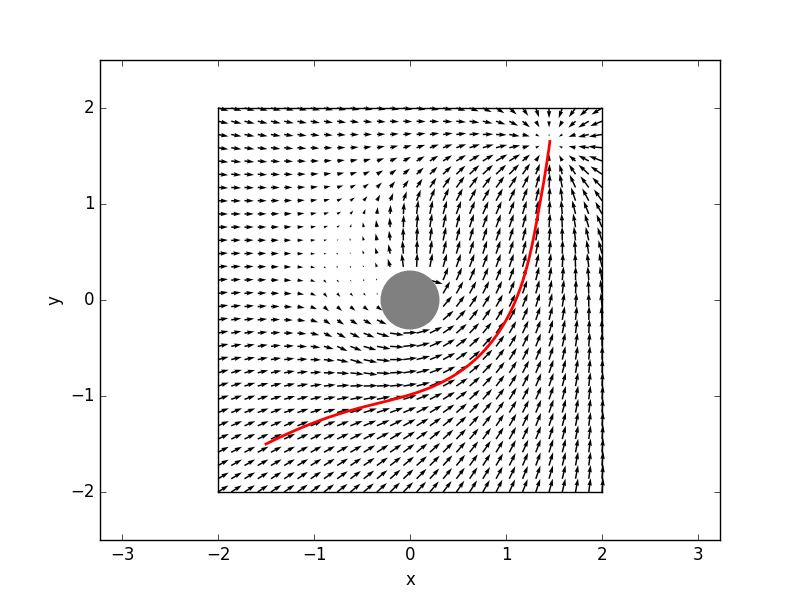
\includegraphics[width=\textwidth]{fig/1e.png}
		\caption{Potential field with the obstacle at (0,0), fixed}
		\label{fig:fixed_potential}
	\end{figure}
	\item The solution from part (e) still works with two obstacles, with the robot taking a similar path as it is repulsed from both the obstacles.
	\begin{figure}[!h]
		\centering
		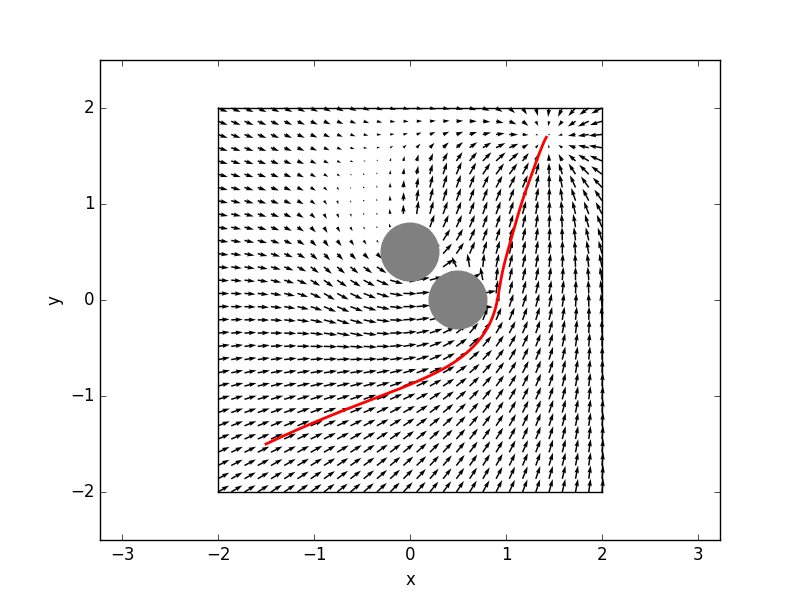
\includegraphics[width=\textwidth]{fig/1f.png}
		\caption{Potential field with two obstacles at (0,0.5) and (0.5,0)}
		\label{fig:fixed_potential}
	\end{figure}
	
\end{enumerate}
\subsection*{Exercise 2}
\begin{enumerate}[label=(\alph*)]
	\item The equations for feedback linearization:
		$$\dot{x_p} = u\cos{\theta} - \epsilon \omega \sin{\theta}$$
		$$\dot{y_p} = u\sin{\theta} + \epsilon \omega \cos{\theta}$$
		Rearranged for $u$ and $\omega$:
		$$ u =x_p\cos{\theta} + y_p\sin{\theta} $$
		$$ \omega = {(-x_p\sin{\theta}+y\cos{\theta})\over{\epsilon}}$$
	\item The point of feedback linearisation is to allow a non-holonomic robot to appear to move holonomically, by controlling a holonomic point and calculating how the robot would move as if 'pulled' by that point.
	\item The plot below shows the trajectory of the robot as it navigates from the start to the goal.
	\begin{figure}[!h]
		\centering
		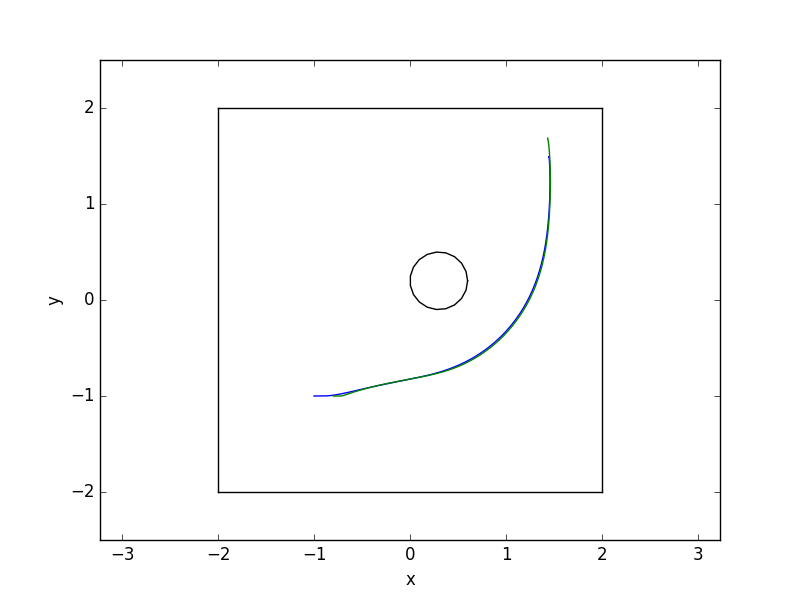
\includegraphics[width=\textwidth]{fig/2c.png}
		\caption{Trajectory of robot in potential field}
		\label{fig:trajectory}
	\end{figure}
	\item 
	\begin{figure}[!h]
		\centering
		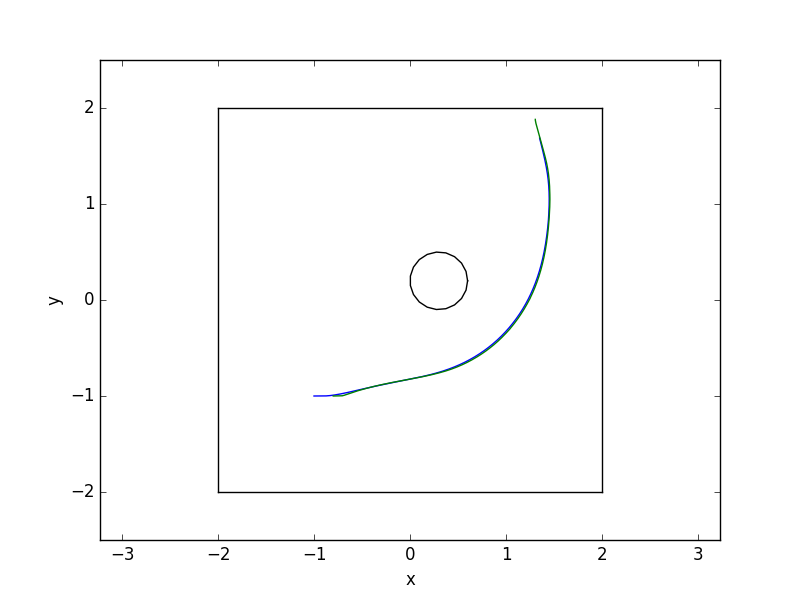
\includegraphics[width=\textwidth]{fig/2d.png}
		\caption{Trajectory of robot in potential field, using relative position}
		\label{fig:trajectory}
	\end{figure}

\end{enumerate}$$
\section*{1.2 Rapidly-Exploring Random Trees}
\subsection*{Exercise 3}
\begin{enumerate}[label=(\alph*)]
	\item 

\end{enumerate}
\subsection*{Exercise 4}
\begin{enumerate}[label=(\alph*)]
	\item 

\end{enumerate}


\end{document}
